\documentclass[11pt]{article}
\usepackage[margin=1in, top=0.3in]{geometry}
\usepackage[all]{nowidow}
\usepackage[hyperfigures=true, hidelinks, pdfhighlight=/N]{hyperref}
\usepackage[separate-uncertainty=true, group-digits=false]{siunitx}
\usepackage{graphicx,amsmath,physics,tabto,float,amssymb,pgfplots,verbatim,tcolorbox}
\usepackage{listings,xcolor,subfig,caption,import,wrapfig}
\usepackage[version=4]{mhchem}
\usepackage[noabbrev]{cleveref}
\newcommand{\creflastconjunction}{, and\nobreakspace}
\numberwithin{equation}{section}
\numberwithin{figure}{section}
\numberwithin{table}{section}
\definecolor{stringcolor}{HTML}{C792EA}
\definecolor{codeblue}{HTML}{2162DB}
\definecolor{commentcolor}{HTML}{4A6E46}
\captionsetup{font=small, belowskip=0pt}
\lstdefinestyle{appendix}{
    basicstyle=\ttfamily\footnotesize,commentstyle=\color{commentcolor},keywordstyle=\color{codeblue},
    stringstyle=\color{stringcolor},showstringspaces=false,numbers=left,upquote=true,captionpos=t,
    abovecaptionskip=12pt,belowcaptionskip=12pt,language=Python,breaklines=true,frame=single}
\lstdefinestyle{inline}{
    basicstyle=\ttfamily\footnotesize,commentstyle=\color{commentcolor},keywordstyle=\color{codeblue},
    stringstyle=\color{stringcolor},showstringspaces=false,numbers=left,upquote=true,frame=tb,
    captionpos=b,language=Python}
\renewcommand{\lstlistingname}{Appendix}
\pgfplotsset{compat=1.17}
\DeclareSIUnit\mevee{MeVee}

\begin{document}

\begin{center}
    {\huge Digital methods for neutron pulse shape discrimination in EJ-301 liquid scintillator detectors}\\
    \vspace{0.2in}
    {\Large Miles Kidson}\\
    \vspace{0.1in}
    {\large Tanya Hutton, Andy Buffler}\\

    \section*{Abstract}\label{sec:Abstract} % rough rn
    Two digital methods of pulse shape discrimination for neutron and gamma-ray events in an EJ-301 scintillator detector are investigated. One has been used extensively historically (CCM) and the other (Pad\'e-Laplace) is tested for the first time. Both methods take advantage of the fact that neutron events in these detectors result in an output signal with a larger contribution from longer time-scale processes than gamma-ray events. Pulse shape discrimination is needed because most neutron detectors are also sensitive to gamma-rays.
    
\end{center}

\section{Introduction}\label{sec:Introduction}
\par Many areas of research rely on the detection of particles, the details of which form the data that is analysed and investigated in order to corroborate or disprove theory. It is very important, when detecting a particle, that you are certain that the particle is what you think it is. When it comes to detecting neutrons, this is not as simple as it sounds. 
\par Liquid scintillator detectors are often used in neutron detection due to their flexibility when it comes to the shape and size of the material as well as their fast timing performance, but these detectors are also sensitive to gamma rays. Scintillator detectors work by emitting light at an energy roughly proportional to the energy of the incident ionising particle, but the constant of proportionality changes depending on the type of particle \cite{Knoll}. This light is then detected by the photoelectric effect and the resulting voltage pulse collected by instrumentation. Different types of particles also result in slightly different voltage pulse shapes. It is this difference that is exploited by pulse shape discrimination techniques. 
\par These techniques were developed at a time where computational power was lacking, as well as expensive, so they were implemented in analogue systems. These systems integrated the voltage over a long and short time window, then took the ratio of the two values. Neutrons interactions result in larger component of the long integral than gamma-ray interactions, so this ratio is different for these two types of interaction. Due to the nature of the electronics needed to integrate these pulses, the analysis had to be performed at run-time, which means the methods available were severely limited. Since computational power is now much more available and affordable, it no longer makes sense to use these analogue systems when the pulses could be captured digitally and analysed later, with much more freedom to experiment with different techniques, using the same data, in order to compare them. There are also more advanced techniques, such as decomposition of the decay curve into its individual exponential components, that are now possible.
\par This report will investigate the digital implementation of a technique similar to the one used in analogue systems, the Charge Comparison Method, as well as a new method that is only possible due to the digitisation of the data: the Pad\'e-Laplace Method. The data from two separate neutron sources, detected with a EJ-301 liquid scintillator detector, will be analysed with these two methods in order to compare them based on the Figure of Merit described in Knoll (2010, p.701). The Charge Comparison Method is well understood and simple to implement but does not perform well at lower energies, so other methods must be investigated.

\section{Theory}\label{sec:Theory}
\subsection{Detecting Neutrons}
\par A distinction must be made between ``fast'' and ``slow'' neutrons as they interact with matter in distinct ways. The neutrons of interest in this paper are fast neutrons, with energies $\gtrsim1$ eV. These interact with matter by collisions, scattering off nuclei and depositing some fraction of their kinetic energy, or by inducing reactions in the target material. Slow neutrons, which are not accounted for in this paper, seem to have a much larger cross section of interaction than fast neutrons, which leads to some interesting applications and physics. The detection mechanisms developed for slow neutrons are thus very different to those used for fast neutrons. \cite{Knoll}
\begin{wrapfigure}{r}{0pt}
    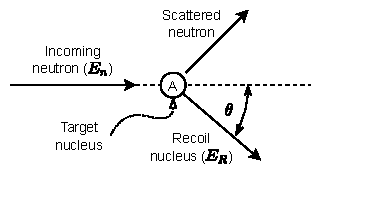
\includegraphics{Plots/neutronScattering.pdf}
    \caption{Elastic neutron scattering.}
    \label{fig:neutron scattering diagram}
\end{wrapfigure}
\par Fast neutrons can be detected in a few different ways, as discussed in Knoll (2010, ch.15), but when the energy of the neutrons is relevant there is only one mechanism of interest: elastic scattering. Neutrons collide with nuclei in the target material and transfer a fraction of their kinetic energy to the nucleus. The fraction of energy deposited is given by
\begin{equation}
    \frac{E_R}{E_n}=\frac{4A}{(1+A)^2}(\cos^2\theta)\;\;\;\cite{Knoll}
    \label{eqn:Neutron scattering fraction}
\end{equation}
where $E_R$ is the energy deposited, $E_n$ is the energy of the incident neutron, $A$ is the mass of the target nucleus in neutron masses, and $\theta$ is the scattering angle of the recoil nucleus, relative to the incoming nucleus.
\par Scintillator detectors work by emitting light as a result of radiation exciting the detector material, whether that's single atoms or creating vibrations in the lattice of the material. Organic scintillator detectors, such as the EJ-301 detector used in this experiment, work by the excitation of single atoms or particles in the detector material. When it comes to neutrons, as seen by \cref{eqn:Neutron scattering fraction}, the mass of the target nuclei affects the fraction of energy that can be absorbed by the detector material. Hydrogen, which has a mass effectively equal to that of a neutron, is thus a very good candidate for absorption of a neutron's kinetic energy by elastic scattering. As a result of this, organic scintillator detectors with a large proportion of hydrogen atoms work well for detecting neutrons, especially when it comes to accurately detecting neutron energy.
\newline
\par When radiation enters the scintillator liquid, due to the so-called $\pi$-electron structure in the material \cite{Knoll}, energy is absorbed by exciting electrons into excited states, which then drop back down to the ground state, emitting light. This $\pi$-electron structure allows for two ``types'' of excitation: singlet (S) and triplet (T) states. The singlet states are quickly de-excited to the ground state with a characteristic lifetime of a few nanoseconds, resulting in what is known as prompt fluorescence. The triplet states, however, have a characteristic lifetime of a few milliseconds, about 6 orders of magnitude difference. When these triplet states de-excite, they emit light of a different wavelength than that of the singlet states so it usually does not contribute to the light output of the scintillator as the materials are often designed to be transparent to only some wavelengths of light. The electrons in triplet states can, however, be thermally excited into singlet states, which will then de-excite and emit the same wavelength as before, but after a longer time than if the electron were immediately in a singlet state. This is called delayed fluorescence.
\par This difference in characteristic time for light output with the same wavelength is the basis of the techniques used to discriminate between gamma-ray and neutron events. Neutrons collide with protons, while gamma-rays collide with electrons. As these charged recoil particles travel through the detector material, its electrons are excited and subsequently light is emitted as they de-excite, but recoil protons and electrons excite the material to the singlet and triplet states in different proportions. Protons tend to excite to triplet states more than electrons do. This means that over the whole interaction, the light output is the same for protons and electrons, but there is more prompt fluorescence for electrons than for protons, and vice-versa for delayed fluorescence. By determining the fraction of delayed to prompt fluorescence for each event, neutron and gamma-ray events can be separated.
\newline
\par The scintillator material, once excited, emits light of a specific wavelength which the material is transparent to. Some of this light will be incident on a plate, called the cathode, which is designed to be efficient at absorbing the light through the photoelectric effect, creating a build-up of electrons. This plate is the start of an array of dynodes, all connected to a high voltage power supply, that will multiply the number of electrons at each step, resulting in a voltage pulse that is detectable. This array of dynodes, ending in an anode, is called a photomultiplier tube (PMT). This pulse is fed through a system of amplifiers until it is captured by a digitiser. The signal can be extracted at different dynodes in the PMT for different purposes. The anode outputs a fast signal which includes the detail needed to discriminate between gamma-ray and neutron events.
\newline
\par Neutrons can, given the right detector material, deposit all of their energy into the recoil particle \cite{Knoll}. The detector, however, is not able to detect this energy exactly. Since the protons are recoiling, not the electrons as it is for gamma-rays, there is a different energy response to neutrons and gamma-rays of the same kinetic energy. Because of this difference, events cannot be compared on simply energy, so a new unit is defined: MeV electron equivalent (MeVee). For gamma-rays, this is equivalent to the standard energy, but for neutrons this is the energy detected by the detector, calibrated with respect to gamma-ray sources such as \ce{^{137}Cs}. This is obviously not the energy of the incident neutron, but the relationship between neutron energy and MeVee's is well understood. 
\par A note must also be made with regards to detected gamma-rays. Due to the material make-up of these detectors, gamma-rays can only deposit their energy by Compton scattering or pair production, but pair production is far less common. This means the energy detected will never be the energy of the gamma-ray, but once again Compton scattering is well understood and shouldn't create any problems. The Compton edge for a gamma-ray of energy $E_\gamma$ is
\begin{equation}
    E_{\mathrm{Compton}} = \frac{2E_\gamma^2}{m_ec^2+2E\gamma}
    \label{eqn:Compton Edge}
\end{equation}

\subsection{Pulse Shape Discrimination Methods}
\par The first method used in this paper is one that has been used extensively in both analogue and digital settings and is in some ways the most simple interpretation of the difference between neutron and gamma-ray events. The characteristic time-scale of prompt fluorescence is a few nanoseconds, while delayed fluorescence has a characteristic time-scale of a few hundred nanoseconds for the EJ-301 detector \cite{Kuchnir}. Knowing this, the signal can be integrated over a short and long time period, corresponding to the prompt and delayed fluorescence time-scales respectively, and the values compared. For neutron events, a larger proportion of the long integral $I_{\mathrm{long}}$ to the short integral $I_{\mathrm{short}}$ is expected compared to that for gamma-ray events. This method is called the Charge Comparison Method (CCM) and the associated discrimination parameter is defined as 
\begin{equation}
    S_{CCM}=\frac{I_{\mathrm{short}}}{I_{\mathrm{long}}}
    \label{eqn:CCM parameter}
\end{equation}

\par The second method used in this paper is a proposed method that considers the fact that the decay of the voltage pulse should be a linear combination of two exponential decays: one associated with the prompt fluorescence, which should have a decay constant much smaller than that of the second, which is associated with the delayed fluorescence. The decay is expected in the form
\begin{equation}
    f(t)=A_pe^{-\lambda_pt}+A_de^{-\lambda_dt}
    \label{eqn:linear exponential combination}
\end{equation}
\par By fitting this function to the signal, the decay constants and their respective amplitudes can be found. This could be done using some nonlinear fitting program such as \texttt{scipy.optimize.curve\_fit} but that runs into issues when it comes to both the time taken per event and the stability of the function; it often runs into issues with bad data that results in it fully stopping the program. For these reasons another method was chosen. 
\newline
\par The Pad\'e-Laplace method of determining exponential time constants in a decaying signal was first described in \cite{Yeramian} but \cite{Hellen-Pade} does a better job of describing the implementation. One feature of this method is that it does not require a hypothesis for the number of exponential terms, but since the theory states that only two terms are expected, this feature will not be used. Nevertheless, the method goes as follows.
\par The decays of interest are those in the form
\begin{equation}
    f(t)=\sum_{i=1}^n A_i e^{\lambda_i t}
    \label{eqn:exponential decay sum}
\end{equation}
where each $A_i$ are the amplitudes and $\lambda_i$ are the decay constants. Note the lack of a minus sign in the exponential. This is for simplicity in the coming calculations and will simply result in a change of sign of the output, which is easily dealt with. The Laplace transform of this function is 
\begin{align}
    \mathcal{L}[f](p)&=\int_0^\infty f(t)e^{-pt}dt\label{eqn:laplace transform}\\
    &=\sum_{i=1}^n\frac{A_i}{p-\lambda_i}\label{eqn:transformed exponential}
\end{align}
\par Here $p$ is some complex number. Clearly the decay constants and respective amplitudes can easily be found by finding the poles and residues of \cref{eqn:transformed exponential}. This, however, is a non-trivial matter and is the reason Pad\'e approximants are used. The Pad\'e approximant needed here is defined, with $L(p)$ being expanded in a Taylor series about $p=p_0$, as
\begin{align}
    P_{n-1,n}(p)&=L(p)\\
    \frac{a_0+a_1(p-p_0)+\dotsi+a_{n-1}(p-p_0)^{n-1}}{1+b_1(p-p_0)+\dotsi+b_n(p-p_0)^n}&=d_0+d_1(p-p_0)+\dotsi+d_{2n-1}(p-p_0)^{2n-1}\label{eqn:pade approximant}
\end{align}
The coefficients on the RHS are 
\begin{align}
    d_i&=\frac{1}{i!}\left(\frac{d^{(i)}L}{dp^{i}}\right)_{p=p_0}\;\;\;(i=0,\dots,2n-1)\\
    &=\frac{1}{i!}\Delta t\left(\frac{1}{2}((-t_1)^ie^{-p_0t_1}f_1+(-t_M)^ie^{-p_0t_M}f_M)+\sum_{j=2}^{M-1}(-t_j)^ie^{-p_0t_j}f_j \right)
\end{align}
where in the last step the Laplace transform of discretised data has been approximated as in \cite{Hellen-Pade} (eqn. 2). From this Taylor series, which is known, the Pad\'e approximants can be found by some algorithm, in this case \texttt{scipy.interpolate.pade} will be used and the coefficients $a_i,\, b_i$ found. Finding the poles $s_i$ and residues $r_i$ can also be done in any appropriate way, so \texttt{scipy.signal.residue} will be used. The decay constants are then simply $\lambda_i=-(s_i+p_0)$ and the associated amplitudes are just $A_i=r_i$.
\par In the case where the number of decay terms is unknown, this process would be repeated starting from $n=1$ until no new poles are found, which is its own interesting problem, but since it is known that there should be two terms, just using $n=2$ is sufficient. The only input required for this method to work is an appropriate choice for $p_0$. \cite{Hellen-Pade} recommends choosing the inverse of the time it takes for the signal to decay to half its initial value, which is easily implemented. 
\par The crux of this method rests on the assumption that there will only be two decay terms, and the ratio of the amplitudes of these terms will vary depending on if the event is a neutron of gamma-ray. For neutron events, the ratio between the amplitudes of the two decay components should be less than that for gamma-rays. Our discrimination parameter is then
\begin{equation}
    S_{PL}=\frac{A_p}{A_d}
    \label{eqn:PL parameter}
\end{equation}

\section{Methodology}\label{sec:Methodology}
\subsection{Experimental Set-up}
\par The two neutron sources used in this experiment were an americium–beryllium (AmBe) source (\SI{2.2}{\giga\becquerel}) which emits neutrons isotropically with energies from $\sim0.025$ eV to $\sim11$ MeV and gamma-rays of $\sim4.4$ MeV, as well as a MP-320 sealed tube neutron generator (STNG), which emits mono-energetic 14 MeV neutrons. The neutrons from the STNG interact with surrounding material, resulting in emitted gamma-rays in a wide range of energies, in this case anything up to $\sim7$ MeV but with a higher energy STNG, this range could increase. 
\par The two sources are housed within a vault of shielding material, with a small channel through which the neutrons can travel towards the detector. The detector is a EJ-301 liquid scintillator detector set at \SI{-1040}{\volt}. The anode of the PMT fed into a CAEN DT5730 digitiser and QtDAQ software. The acquisition window was set to \SI{3}{\micro\second} and the trigger set to the anode showing a voltage above the threshold of \SI{0.2}{\volt}.
\begin{table}[H]
    \centering
    \begin{tabular}{c|c}
        Source & Acquisition time \\ \hline
        STNG (HV 80 kV, BC \SI{60}{\micro\ampere}) & \SI{1545}{\second} \\\hline
        AmBe (\SI{2.2}{\giga\becquerel}) & \SI{201}{\second}\\\hline
        \ce{^{22}Na} & \SI{107}{\second}\\\hline
        \ce{^{137}Cs} & \SI{127}{\second}\\\hline
        \ce{^{60}Co} & \SI{215}{\second}
    \end{tabular}
    \caption{The data taken for this experiment. Acquisition time for each is shown, along with the relevant settings for each source. The last three sources were used for calibration. Data taken by T. Hutton, A. Buffler, and S. Mhlongo on 10 August 2021.}
    \label{tbl:data taken}
\end{table}

\subsection{Calibration}
\par Before any analysis of neutrons and gamma-rays can begin, the set-up needs to be calibrated. To do this, radioisotopes with known energy gamma-ray emissions were placed in front of the detector and data taken for $\sim150$ seconds. Each event's signal was integrated over the long window and a pulse energy spectrum was created. This data did not show a photopeak, as is expected, but the long integral value for each Compton edge could be extracted for each source. These values could then be correlated to the expected value of the Compton edge and calibration parameters found with a linear least squares fit. 

\begin{table}[H]
    \centering
    \begin{tabular}{c|c|c|c}
        Source & Gamma-ray energy (MeV) & Compton edge energy (MeV) & Long integral value \\ \hline
        \ce{^{22}Na} & \SI{0.511}{\mega\electronvolt} & \SI{0.341}{\mega\electronvolt} & 0.345 \\ 
         & \SI{1.275}{\mega\electronvolt} & \SI{1.062}{\mega\electronvolt} & 1.104 \\ \hline
         \ce{^{137}Cs} & \SI{0.662}{\mega\electronvolt} & \SI{0.477}{\mega\electronvolt} & 0.488 \\ \hline
         \ce{^{60}C0} & \SI{1.332}{\mega\electronvolt} & \SI{1.118}{\mega\electronvolt} & 1.148
    \end{tabular}
    \caption{Data used to calibrate the detector set-up. A linear least squares fit was made using the long integral values on the x-axis and Compton edge energy on the y-axis. The relationship was found to be $E_\gamma=0.92 I_{\mathrm{long}} + 0.0058$ \unit{\mevee}. Gamma-ray energies from \cite{22Na Decay}, \cite{137Cs Decay}, and \cite{60Co Decay}. Compton edges calculated with \cref{eqn:Compton Edge}.}
    \label{tbl:Calibration Sources}
\end{table}

\par Now when the long integral is taken for any event, it can be assigned an energy in units of \unit{\mevee}, no matter if it's a neutron or gamma-ray event. This energy is defined as a new parameter $L$ so as not to confuse it with actual energy, since they are subtly different. 

\subsection{Implementation of Discrimination Methods}
\begin{wrapfigure}{r}{0.5\textwidth}
    \scalebox{0.5}{\subimport{Plots}{anode_no_flip.pgf}}
    \caption{An example of the raw data coming from the fast anode with the STNG as a source.}
    \label{fig:anode_no_flip}
\end{wrapfigure}

\par The files output by the QtDAQ system are too big to import in one go, so code written by Chlo\'e Sole was used to extract one event at a time using \texttt{numpy.frombuffer} in the form of a voltage pulse. This pulse was originally in the form of \cref{fig:anode_no_flip}, but this can easily be transformed to a pulse starting at 0 and increasing in voltage: The digitizer always includes 25\% of the total capture window (in this case that's 750 ns) before the trigger event. This should have no relevant signal and so can be averaged to find a baseline voltage which can be subtracted from the entire pulse and then the pulse can be flipped about the horizontal to get it in the form of \cref{fig:anode_flipped}.
\par Once in this form, the pulse can be integrated over the two windows shown using \texttt{np.trapz} and the discrimination parameter calculated using \cref{eqn:CCM parameter}. To begin, the long and short windows were chosen to be \SI{250}{\nano\second} and \SI{20}{\nano\second} respectively to include the delayed and prompt fluorescence respectively. These specific values were chosen because they have been used historically in the neutron lab at UCT. The long window was left untouched but the short window length needed to optimised.

\par In order to optimise the window length, the notion of a good discrimination is needed. To do this, the traditional Figure of Merit (FoM) from Knoll (p.701) is used. The events are histogrammed by their discrimination parameter $S_{\mathrm{CCM}}$ and two peaks should be seen, representing gamma-rays and neutrons (\cref{fig:CCM_AmBe_separation_hist}). The difference in $S_{\mathrm{CCM}}$ between the peaks, divided by the sum of their FWHM's, is the FoM, called $M$:

\begin{equation}
    M = \frac{|x_\gamma-x_n|}{FWHM_\gamma + FWHM_n}
    \label{eqn:Figure of Merit}
\end{equation}
This value will be used throughout this paper to evaluate the quality of the discrimination method. Higher is better. By calculating this $M$ for a range of short integral lengths, an optimal length of \SI{22}{\nano\second} was found. With this optimised short integral window length, the CCM can be used to analyse the data from both the AmBe and STNG sources. 

\begin{wrapfigure}{r}{0.5\textwidth}
    \scalebox{0.5}{\subimport{Plots}{anode_flipped.pgf}}
    \caption{Example of the data used to perform the discrimination methods. The time range has been reduced to better show the details of the pulse. The long and short integral windows are shown, both starting from the same place. }
    \label{fig:anode_flipped}
\end{wrapfigure}

\par The Pad\'e-Laplace method appears to be untested in literature for this application. Even just the method of decomposition into exponential decay components is very lacking, so there is no precedent for the implementation. The author of \cite{Hellen-Pade} has implemented this method in Python to study the decay of a voltage from a simple circuit and the code used in this paper is adapted from his (\cite{Hellen-Code}), using the \texttt{scipy.interpolate.pade} and \texttt{scipy.signal.residue} methods instead of his hardcoded methods which do the same thing, but there are some aspects of this application which could be too much for the method to handle. 

\par Once the decay constants and their associated amplitudes were obtained, the implementation of \cref{eqn:PL parameter} was fairly simple. The only quirk came from the fact that this method does not provide the poles and residues in the same order every time, so adjustments had to be made in order to always compute \cref{eqn:PL parameter} such that the amplitude in the numerator always corresponded to the largest (in absolute value) decay constant as that would be the faster decay, i.e. the prompt fluorescence. 

\section{Results and Analysis}\label{sec:Results and Analysis}
\subsection{Charge Comparison Method}
\par \Cref{fig:CCM_AmBe_hist2d} shows the so-called $L-S$ plot for the AmBe source. There are clearly two distinct loci that we can associate with neutron and gamma-ray events respectively. The theory states that the top locus is gamma-rays and the bottom for neutrons, and this can be further verified by looking at the well defined edge of events around \SI{4.2}{\mevee}. The AmBe source radiates \SI{4.4}{\mega\electronvolt} gamma-rays, so it is expected to see a hard edge associated with that decay mode. Given that this detector only detects gamma-rays through Compton scattering, the maximum energy that can be deposited by a gamma-ray of energy $E_\gamma$ is given by \cref{eqn:Compton Edge}. For this gamma-ray, that should be around \SI{4.159}{\mevee} (given these are gamma-ray events, that is equivalent to \SI{4.159}{\mega\electronvolt}). 
\par After generating an $L-S$ plot, the FoM for this method needs to be determined. Using the parameters found when fitting the functions in \cref{fig:CCM_AmBe_separation_hist}, the separation and FWHM's can easily be found, resulting in an FoM of $M=1.54$. This is acceptable, but it can be improved. In \cref{fig:CCM_AmBe_hist2d}, the separation between neutrons and gamma-rays becomes messy below $L\approx\SI{0.3}{\mevee}$, so by isolating chunks of \SI{2}{\mevee} an FoM can be calculated for each section: 

\begin{figure}[H]
    \begin{center}
        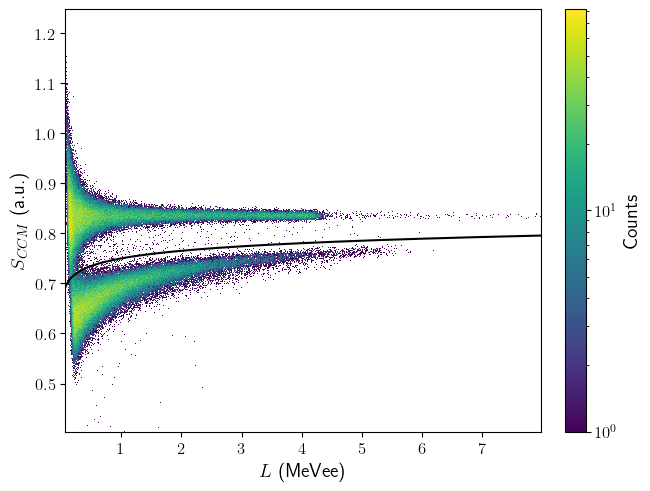
\includegraphics[scale=0.75]{Plots/CCM_AmBe_hist2d.png}
        \caption{2D histogram showing the discrimination parameter $S$ versus the energy $L$ for the AmBe source, analysed using CCM. The plot has been cropped to best show off the relevant parts: the two loci. Above the black line are the gamma-ray events and below the neutron events. The separation was made by trial and error using a log function. Note the defined edge of the gamma-ray locus around \SI{4.2}{\mevee}.}
        \label{fig:CCM_AmBe_hist2d}
    \end{center}
\end{figure}
\begin{figure}[H]
    \begin{center}
        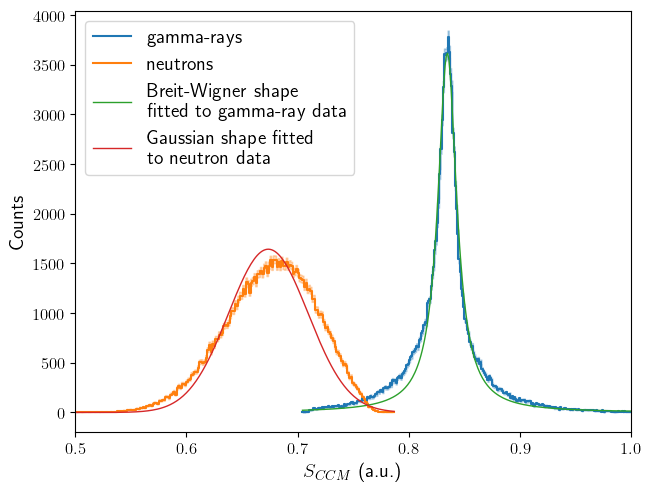
\includegraphics[scale=0.75]{Plots/CCM_AmBe_separation_hist.png}
        \caption{Histograms of the counts per discrimination parameter for the neutron and gamma-ray events from the AmBe source, separated by the black line in \cref{fig:CCM_AmBe_hist2d}. The counts are assumed to be Poisson distributed, so their uncertainties are simply $u(N)=\sqrt{N}$, shown above and below the data. The distributions chosen to fit the data were based purely on what they looked most similar to.}
        \label{fig:CCM_AmBe_separation_hist}
    \end{center}
\end{figure}

\begin{figure}[h]%
    \centering
    \subfloat[\centering $L=$\SI{0}{\mevee} to $L=$\SI{2}{\mevee}. $M=1.64$.]{\scalebox{0.4}{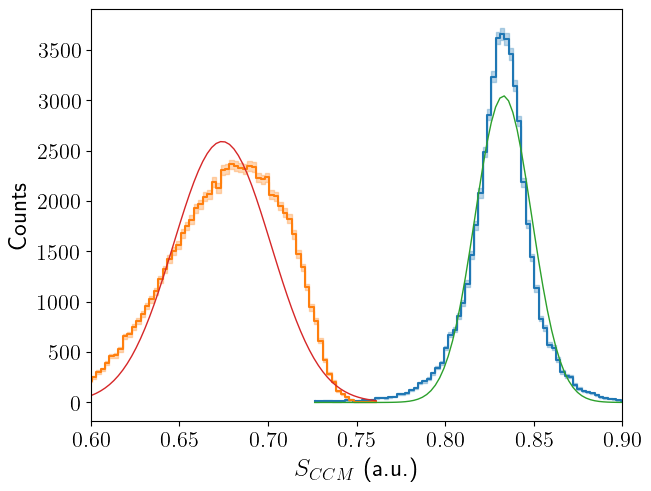
\includegraphics{Plots/CCM_AmBe_separation_hist_2.png}}}
    \,
    \subfloat[\centering $L=$\SI{2}{\mevee} to $L=$\SI{4}{\mevee}. $M=2.62$.]{\scalebox{0.4}{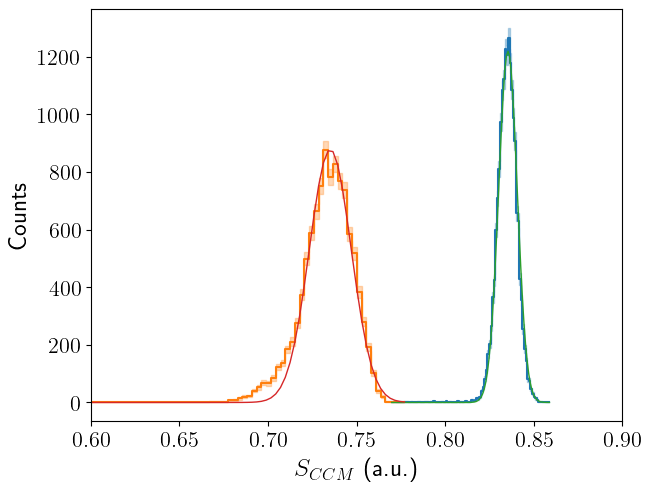
\includegraphics{Plots/CCM_AmBe_separation_hist_4.png}}}
    \caption{Counts per discrimination parameter for two ranges of $L$. The functions fitted are Gaussians. Uncertainties assumed to be Poissonian.}
    \label{fig:CCM_AmBe_separation_hist_split}
\end{figure}
\par Clearly, \cref{fig:CCM_AmBe_separation_hist_split} shows how the lower energy events result in a lower FoM. This can even be seen by looking at the fits. The expected shape of these histograms is a Gaussian since in theory neutrons should always return the same $S$ value, as should gamma-rays. This is clearly not the case at low energies, but at higher energies the Gaussian fits better. 
\par To get a full picture of CCM, the STNG source must be examined as well. 

\begin{figure}[H]
    \begin{center}
        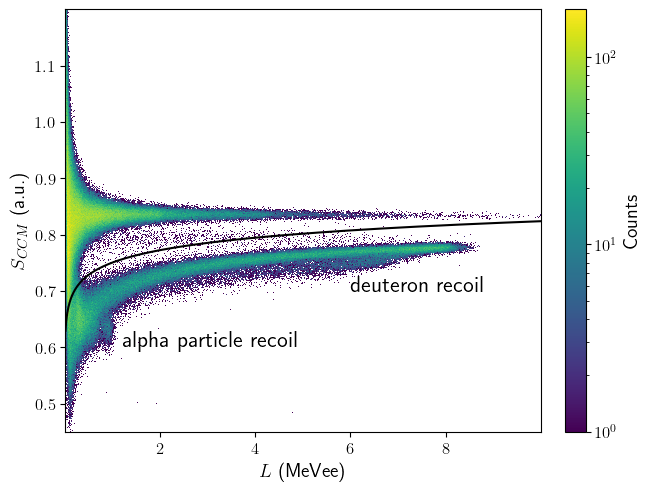
\includegraphics[scale=0.75]{Plots/CCM_STNG_hist2d.png}
        \caption{2D histogram showing the discrimination parameter $S$ versus the energy $L$ for the STNG source, analysed using CCM. The plot has been cropped to best show off the relevant parts: the two loci. Above the black line are the gamma-ray events and below the neutron events. The separation was made by trial and error using a log function. Note the defined edge of the neutron locus around \SI{8}{\mevee}, as well as the two clumps corresponding to deuteron and alpha particle recoils.}
        \label{fig:CCM_STNG_hist2d}
    \end{center}
\end{figure}

\begin{figure}[H]
    \begin{center}
        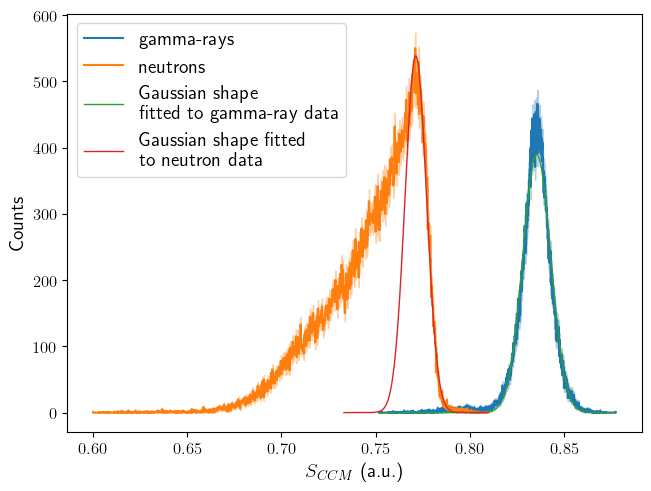
\includegraphics[scale=0.75]{Plots/CCM_STNG_separation_hist.png}
        \caption{Histograms of the counts per discrimination parameter for the neutron and gamma-ray events from the STNG source, separated by the black line in \cref{fig:CCM_STNG_hist2d} and for energies $L>\SI{1}{\mevee}$. The counts are assumed to be Poisson distributed, so their uncertainties are simply $u(N)=\sqrt{N}$, shown above and below the data. The neutron fitting was performed on only the data to the right of the maximum. The FoM was found to be $M=2.27$.}
        \label{fig:CCM_STNG_separation_hist}
    \end{center}
\end{figure}
\par \Cref{fig:CCM_STNG_hist2d} looks, for the most part, just like \cref{fig:CCM_AmBe_hist2d}, but there are a few key differences. The STNG emits \SI{14.1}{\mega\electronvolt} neutrons and a wide spectrum of gamma-rays, so a hard cut is seen around \SI{8}{\mevee} for the neutrons, which is expected given the relationship between \unit{\mevee} and neutron energy \cite{Mevee}. As a result of the high energy neutrons, deuteron and alpha particle recoil events, as opposed to protons, begin to emerge. 
\par This is interesting, but unfortunately it muddies the waters a little bit, as can be seen in \cref{fig:CCM_STNG_separation_hist}: The neutrons seem to have a long tail stretching off into the low $S$ values as a result of these new processes. For this reason, in order to determine the FoM only the right hand side of the distribution was used. These were also only the events of an energy greater that \SI{1}{\mevee} as below that it is much more difficult to separate neutrons and gamma-rays. 

\subsection{Pad\'e-Laplace Method}
\par The long and short of the Pad\'e-Laplace Method is that it did not give the expected results. 



% DON'T FORGET TO CHANGE FROM PNG TO PDF IF YOU FEEL LIKE IT, OR NOT IDC

\begin{thebibliography}{9}
    \bibitem{Knoll}
    G. F. Knoll, \textit{Radiation Detection and Measurement}, 4th ed., Wiley, New York, (2010)

    \bibitem{Lang}
    R. F. Lang, D. Masson, J. Pienaar, and S. R\"ottger, `Improved pulse shape discrimination in EJ-301 liquid scintillators', \textit{Nuclear Instruments and Methods in Physics Research Section A: Accelerators, Spectrometers, Detectors and Associated Equipment} \textbf{856}, 26-31, (2017)

    \bibitem{Kuchnir}
    F. T. Kuchnir and F. J. Lynch, `Time Dependence of Scintillations and the Effect on Pulse-Shape Discrimination,', \textit{IEEE Transactions on Nuclear Science} \textbf{vol. 15, no. 3}, 107-113, (1968).

    \bibitem{Yeramian}
    E. Yeramian and P. Claverie, `Analysis of multiexponential functions without a hypothesis as to the number of components', \textit{Nature} \textbf{326}, 169–174, (1987).

    \bibitem{Hellen-Pade}
    E. Hellen, `Pad\'e–Laplace analysis of signal averaged voltage decays obtained from a simple circuit', \textit{American Journal of Physics} \textbf{73}, 871-875, (2005)
    
    \bibitem{Hellen-Code}
    E. Hellen, Pad\'e-Laplace code in python2.7 as implemented in 2005 AJP article, \url{https://www.researchgate.net/publication/337032883_Pade-Laplace_code_in_python27_as_implemented_in_2005_AJP_article}, (2019)

    \bibitem{22Na Decay}
    M. Shamsuzzoha Basunia, Nuclear Data Sheets 127, 69, (2015)
    
    \bibitem{137Cs Decay}
    E. Browne, J. K. Tuli, Nuclear Data Sheets 108, 2173, (2007)
    
    \bibitem{60Co Decay}
    E. Browne, J. K. Tuli, Nuclear Data Sheets 114, 1849, (2013)

    \bibitem{Mevee}
    A. Aksoy, `Response-function measurement of an NE213 scintillator using the \ce{^2H(d,n)^3He} reaction', \textit{Nuclear Instruments and Methods in Physics Research Section A: Accelerators, Spectrometers, Detectors and Associated Equipment} \textbf{337}, 486-491, (1994)


\end{thebibliography}

\end{document}